\documentclass[12pt,oneside,openany,a4paper,%..... Layout
               afrikaans, 
               english,%.............. Global language selection
               ]{memoir}

 \usepackage[masters-t,%.......................... Master thesis
             goldenblock,%........................ A5 type block (or a5block or wide)
            ]{usthesis}%.......................... US thesis style with memoir

%
% PLEASE read the USthesis documentation for the class options
% and how to set line and paragraph spacing
%

%==== Language setup ================================================
 \usepackage[latin1]{inputenc}%................... Recognizes �, �, etc
 \usepackage{babel}%.............................. Language setup

%==== Math setup ====================================================
 \usepackage{amsmath}%............................ Advanced math (before fonts)
 \usepackage{amssymb}%............................ AMS Symbol fonts

%==== Font setup (default is Computer Modern) =======================
 \usepackage[T1]{fontenc}%........................ Type 1 fonts
 %\usepackage{fourier}
 \usepackage{textcomp}%........................... Additional text character
 \usepackage{bm}%................................. Bold math symbols (after fonts)
 \usepackage{soul}

%==== Ref's, Bib's and Nomencl ======================================
 \usepackage{usnomencl}%.......................... List of symbols (in usthesis pack)
 \usepackage{usbib}%.............................. Bibliography    (in usthesis pack)
    \bibliographystyle{usmeg-a}
    \renewcommand\bibfont{\small}

    %% For usmeg-a, the bib is a list of references. If you
    %% are using usmeg-n comment out the following lines
    %\addto{\captionsafrikaans}{\renewcommand{\bibname}{Lys van Verwysings}}
    \addto{\captionsenglish}{\renewcommand{\bibname}{List of References}}

%==== Graphics and Color ============================================
\usepackage{graphicx}%........................... Graphicx loaded in usthesis
\usepackage{color}%.............................. Color setup
\usepackage{eso-pic}%............................ Shipout commands for watermark
    \newcommand*{\WaterMark}[2][0.15\paperwidth]{%
        \AddToShipoutPicture*{\AtTextCenter{%
                \parbox[c]{0pt}{\makebox[0pt][c]{%
                    \includegraphics[width=#1]{#2}}}}}}

%==== Local Defs ====================================================
\makeatletter

%
% Please insert user defined commands here

\usepackage{hyperref}
\graphicspath{figs/}

\usepackage{array}
\usepackage{ragged2e}
\usepackage{longtable}
\usepackage{booktabs}
\usepackage{multirow}
\usepackage{subcaption}
\usepackage{float}
\floatstyle{plaintop}
\restylefloat{table}
\usepackage{rotating}
\usepackage{pdflscape}
\usepackage{siunitx}

% and NOT in the document itself!
%

\makeatother

%==== TITLE PAGE ====================================================
\title{\bfseries
       \AorE{%-- Afrikaans ------------------------------------------
             'n Skaal-Onafhanklike Generatiewe Ontwerpproses vir 2D Sagte Robotaktore\\[1ex]
             \normalfont\small\itshape
             (``A Scale-Invariant Generative Design Process for 2D Soft Robot Actuators'')
            }{%-- English -------------------------------------------
             A Scale-Invariant Generative Design Process for 2D Soft Robot Actuators
            }}

\author{N. T.\ Conradie}{Naud\'e Thomas Conradie}

\degree{\AorE{MIng (Meg)}{MEng (Mech)}}
       {\AorE{Magister in Ingenieurswese (Megatroniese)}
             {Master of Engineering (Mechatronic)}}

%\address{\AorE{%-- Afrikaans ----------------------------------------
%        Departement Meganiese en Megatroniese Ingenieurswese,\\
%        Universiteit van Stellenbosch,\\
%        Privaatsak X1, Matieland 7602, Suid Afrika.%
%             }{%-- English ------------------------------------------
%        Department of Mechanical and Mechatronic Engineering,\\
%        University of Stellenbosch,\\
%        Private Bag X1, Matieland 7602, South Africa.
%            }}

\faculty{\AorE{Fakulteit Ingenieurswese}%
              {Faculty of Engineering}}

\supervisor{Dr.\ M. P.\ Venter}
%\cosupervisor{Mnr.\ J.\ Smith}

\setdate{04}{2021}

%\SetSponsor{The financial assistance of the National Research Foundation (NRF)
%    towards this research is hereby acknowledged. Opinions expressed and
%    conclusions arrived at, are those of the author and are not necessarily to
%    be attributed to the NRF.}


%====================================================================
%     MAIN DOCUMENT
%====================================================================
\maxsecnumdepth{subsubsection}
\maxtocdepth{section}

\begin{document}

%==== Front matter ==================================================
 \frontmatter
% \WaterMark{UScrest-WM}
 \TitlePage

 \DeclarationDate{2020/11/20}
 \DeclarationPage
 \clearpage

 \begin{abstract}[english]%===================================================

\end{abstract}


%\begin{abstract}[afrikaans]%=================================================

%\end{abstract}


\chapter{Acknowledgements}%==================================================

I would like to express my sincere gratitude to the following people and organisations:

Doctor Martin Venter, my supervisor and co-author, for his assistance and patience throughout this project

De Beers Marine Namibia, for sponsoring my studies



\chapter{Dedications}%=======================================================
 \vfill
 \begin{center}\itshape
 	I would like to dedicate this thesis to my wife, Anmari Conradie, for her support and understanding throughout this project.
 \end{center}
 \vfill
 \clearpage

%============================================================================
\endinput


 \tableofcontents
 \clearpage

 \setcounter{lofdepth}{2}
 \listoffigures
 \clearpage

 \listoftables
 \clearpage

% \chapter{Nomenclature}

\begin{Nomencl}
 \NomGroup{Constants}%-----------------------------------------------
   \item[$\mathrm{g} = $] $\mathrm{9.81\,m/s^2}$

 \NomGroup{Variables}%-----------------------------------------------
   \item[$\mathit{Re}_\mathrm{\,D}$]
                      \UnitLine{Reynolds number (diameter)}{~}
   \item[$x$]         \UnitLine{Coordinate                }{m}
   \item[$\ddot{x}$]  \UnitLine{Acceleration              }{m/s^2}\\
   \item[$\theta$]    \UnitLine{Rotation angle            }{rad}
   \item[$\tau$]      \UnitLine{Moment                    }{N{\cdot}m}

 \NomGroup{Vectors and Tensors}%-------------------------------------
   \item[$\overrightarrow{\bm{v}}$] Physical vector, see equation ...

 \NomGroup{Subscripts}%----------------------------------------------
   \item[$\mathrm{a}$] Adiabatic
   \item[$a$]          Coordinate
\end{Nomencl}



\endinput


%==== Main document =================================================
\mainmatter
   \setsecnumdepth{subsubsection}
%   \numberwithin{equation}{section}
%   \numberwithin{figure}{chapter}
%   \numberwithin{table}{chapter}

\chapter{Introduction}
\label{chp:I}

%%%%%%%%%%%%%%%%%%%%%%%%%%%%%%%%%%%%%%%%%%%%%%%%%%%%%%%%%%%%%%%%%%

\section{Background}

Manufacturing capabilities have greatly increased over the past decades. The advent of three dimensional (3D) printing and other advanced manufacturing technologies have allowed for the production of novel geometries that were previously unattainable. \citep{Buchanan2019,Luis2020}

Development of new products and systems may now be limited by current design capabilities of humans. Improving and creating new design methods may lead to innovative designs not yet seen before. Design methods involving collaboration with computers executing generative design procedures allows for exploration of complex geometries. \citep{Shea2005}

The field of soft robotics is particularly suited to creative and novel approaches to the design of components. Soft robotic geometries are often highly complex and free-form. Soft robotic actuators may move in imprecise and non-trivial manners \citep{Whitesides2018}. Materials used in the construction of soft robotic components may behave with non-linear responses \citep{Boyraz2018}. Novel soft robotic actuator designs with new and non-trivial behaviours are actively being created and implemented \citep{Ellis2020}.

A computationally efficient generative design approach may be used to explore the design space of soft robotics. Hyper-elastic non-linear material models are computationally expensive. Simplifying the model representation or evaluation is thus desirable \citep{Niroomandi2010}. Generative design is a powerful automated approach to design that evaluates the performance of many different potential design solutions. Generative design is useful when performing manual design evaluations becomes tedious or impossible within realistic time constraints \citep{Brose1993}.

\section{Aim and Objectives}

The aim of this project is to implement a scale-invariant generative design process that results in replicable soft robotic actuator components. A scale-invariant process would allow for an efficient encoding that can be applied to a wide range of resolutions yielding similar performances. A generative design process would entail a computationally focused design process with initial parameters defined by a human user, the design process largely carried out independently by the software pipeline and appropriate designs selected and refined by the user. The design process should be compatible with multiple objective functions for the actuators. The design software should be easily modifiable and adaptable. To this end, the project's objectives are outlined as:

\begin{enumerate}
	\item Review existing approaches to modelling and designing soft bodies to determine appropriate methods to be investigated
	\item Implement a scale-invariant generative design process capable of generating manufacturable soft robotic actuator components fulfilling a given objective function
	\item Verify the simulated performance of generated bodies by constructing and examining a physical model
\end{enumerate}

\section{Scope and Assumptions}
\label{sec:SaA}

Some assumptions are made to reasonably limit the scope of the project:

\begin{enumerate}
	\item The design approach will be generalised as much as possible to allow for easy modification of physical dimensions, material properties and objective functions
	\item The design approach will be limited to the consideration of soft materials
	\item The design space will be limited to 2D solutions
	\item Existing FEM software will be used for material modelling
\end{enumerate}

\section{Project Overview}

Chapter~\ref{chp:LR} consists of a literature review exploring the field of soft robotics in general, as well as focusing on soft robotic actuators and design approaches. The literature review also discusses generative design approaches including genetic algorithms, Monte Carlo simulations, L-Systems, and CPPNs. A short discussion on the phenomenon of emergent properties is also included. Chapter~\ref{chp:MaM} encapsulates the materials and methods relevant to this project. The materials used in the simulation and practical testing thereof are discussed. The generative design methods as applied are discussed in detail. The software implementation is elaborated upon. Chapter~\ref{chp:R} discusses results obtained from running simulations according to specified parameters. Chapter~\ref{chp:MV} showcases a physical replication of models generated during the simulations. A conclusion to the project is presented in Chapter~\ref{chp:C}.
\chapter{Literature Review}
\label{chp:LR}


%%%%%%%%%%%%%%%%%%%%%%%%%%%%%%%%%%%%%%%%%%%%%%%%%%%%%%%%%%%%%%%%%%%%%%%
\section{Soft Robotics}

The field of soft robotics is relatively new and developmental. Soft robots inherently differ from traditional robots. They are constructed from compliant and pliable materials. Soft robots generally have fixed joints and locomotive actuators between joints, as opposed to traditional robots which usually have locomotive actuated joints connected by rigid sections. \cite{Whitesides2018}

Soft robots offer many advantages over traditional robots. They provide a safer working environment around humans and with fragile materials, as they are much lighter, more pliable and move slower and with less force than traditional robots. They require lower tolerances for manufacture due to their inherent less precise nature. The fact that they are very lightweight relative to traditional robots may also offer many advantages. \cite{Whitesides2018}

\subsection{Actuators}

Actuators are components that cause controlled motion, generally used in robotics and machinery \cite{Sekhar2012}. There are currently a few major types of soft robotic actuators in use \cite{Boyraz2018}.

\subsubsection{Actuator Types}

Shape Memory Alloys (SMA) are metallic alloys capable of being formed into a specific shape while above an inherent transformation temperature, as well as being formed into another shape below the transformation temperature. When the material is then heated or cooled above or below the transformation temperature, it reforms into those respective shapes. This property exists due to the transition between the martensite phase of the material below the transformation temperature, and the austenite phase above the transformation temperature. SMA actuators are heated by applying a current directly to the material. SMA actuators are small, lightweight, silent, and have a high force-to-weight ratio. When shaped straight, they can exert high forces, but only achieve small displacements relative to their length. When coiled, they can extend more, but exert smaller forces. \cite{Villoslada2015}

\hl{insert illustrative figure}

Shape Memory Polymers (SMP) are similar to SMAs, consisting of smart polymers with the same shape memory properties, instead of metallic alloys. The initial is shape is determined during the manufacturing process. The transformed shape is obtained by cooling the SMP and shaping it as desired. SMPs use electricity or light as a heat source for transformation \cite{Behl2207}. They have a high deformation capacity and shape recovery. They are lighter, cheaper and easier to produce than SMAs. They are limited in size due to their low recovery stresses {Rodriguez2016}.

Dieelectric/Electrically-Actuated Polymers (DEAP) consist of layers of polymers interspersed with conductive material. When the conductive material receives an electrical input, a chemical reaction occurs that causes a change in volume across the layers. This causes the layers to bend in a predetermined direction. DEAPs are lightweight, silent and use little energy. They are biocompatible and functional in water. They are well-suited to mimicking real muscles. Their reactions under high voltages are not fully understood yet and accurately modelling them is highly complicated. \cite{Mutlu2014}

Electro-Magnetic Actuators (EMA) make use of magnetic microparticles within a polymer matrix. The particles are manipulated to cause motion by an external magnetic field from an electromagnet. This allows for a wide range of motion by varying the orientation and magnitude of the electromagnetic field. EMAs are small, require low voltages and are efficient. They have quick response times and high dynamic ranges. They are still an emerging technology in the early stages of development. \cite{Do2018}

Fluid Elastomeric Actuators (FEA) use soft polymeric structures with internal geometry designed for specific types of motion when driven by fluid pressure. Fluid pressure may be obtained from pressurized containers or chemical reactions. They are simple to design, manufacture and control, and are lightweight and usually inexpensive. They are scalable to different sizes and resistant to many types of damage. \cite{Shepherd2011,Onal2017}.

\subsubsection{Actuator Shapes}

\hl{linear extension and resulting motion and application}

\hl{torsional extension and resulting motion and application}

FEAs can be built to curl while contracting and straighten out while expanding, similar to natural muscles. This has a range of applications, especially when multiple of these FEAs are used in conjunction with one another. One application is as a gripper, where a number of these FEAs are arranged similarly to a hand or tentacles all curling inward. Grippers are well-suited to picking up and manipulating soft and/or irregularly shaped objects.

\hl{insert diagrams}

%%%%%%%%%%%%%%%%%%%%%%%%%%%%%%%%%%%%%%%%%%%%%%%%%%%%%%%%%%%%%%%%%%%%%%%
\section{Soft Robot Modeling}

\subsection{Modeling Approaches}

\hl{discuss FEM, voxels, tetrahedral meshes and Gaussian distribution}

\subsection{Modeling Software}

\hl{discuss software options}

%%%%%%%%%%%%%%%%%%%%%%%%%%%%%%%%%%%%%%%%%%%%%%%%%%%%%%%%%%%%%%%%%%%%%%%
\section{Evolved Virtual Bodies}

\subsection{Generative Design}

\subsubsection{Evolutionary Algorithms}

\hl{discuss evolutionary algorithms}

Evolutionary algorithms require a measure of the population's performance. Within the context of evolving simulated physical bodies, a realistic physically simulated goal is usually set. Examples include traversing the greatest distance within a set amount of time, jumping or climbing over an obstacle, or drawing another object closer to it. Fitness measures may also be implemented as survival criteria in testing, such as energy requirements, size, and complexity of the respective bodies. \cite{Sims1994a, Sims1994}

\subsubsection{Lindenmayer Systems (L-systems)}

\hl{discuss L-systems}

\subsubsection{Compositional Pattern Producing Networks (CPPN)}

\hl{discuss CPPNs)

\subsubsection{Emergent Properties}

Emergent properties are sometimes encountered with generative design. Emergent properties may be complex behaviours that are challenging to understand initially, that arise from the combination of the simple elements and rules used to construct the generative design algorithms. For example, virtually evolved bodies may end up being complexly constructed in such a way that the methods of completing their objectives are not initially obvious \cite{Damper2000}. These emergent properties are desirable, as one advantage of generative design processes is that they may arrive at original and unique designs that may be extremely difficult for a human to arrive at \cite{Sims1994a}.

\subsection{Previous Attempts}

\hl{discuss previous attempts}


\chapter{Material Testing}
\label{chp:MT}

%%%%%%%%%%%%%%%%%%%%%%%%%%%%%%%%%%%%%%%%%%%%%%%%%%%%%%%%%%%%%%%%%%%%%%%
\section{Motivation}

\subsection{Material}

Mold Star 15 SLOW is selected as the main material to be digitally modelled for the purposes of the project. Mold Star 15 is selected because of its availability and properties. Mold Star 15 is deliverable to the premises where testing is to be done and available from a registered supplier. Additional properties are listed in~\ref{tab:gmp} below.

\begin{table}[h]
	\centering
	\caption{Given Material Properties}
	\label{tab:gmp}
	\resizebox{\textwidth}{!}{%
		\begin{tabular}{@{}ccccc@{}}
		\toprule
		\textbf{Material} & \textbf{Cost/kg} & \textbf{Pot life (min)} & \textbf{Cure time (hr)} & \textbf{Tensile strength (MPa)} \\ \midrule
		Mold Star 15 SLOW & R332.00 & 50 & 4 & 2.7579 \\ \bottomrule
		\end{tabular}%
	}
\end{table}


\subsection{Testing}

Standardised testing of the materials to be modelled digitally is done in order to obtain accurate physical properties. The necessary properties to model the material chosen 
\chapter{Results}
\label{chp:R}

%%%%%%%%%%%%%%%%%%%%%%%%%%%%%%%%%%%%%%%%%%%%%%%%%%%%%%%%%%%%%%%%%%%%%%%



\chapter{Model Validation}
\label{chp:MV}

%%%%%%%%%%%%%%%%%%%%%%%%%%%%%%%%%%%%%%%%%%%%%%%%%%%%%%%%%%%%%%%%%%%%%%%

Physical replicas of selected units are constructed and inflated. The deformation is observed and compared with the modelled behaviour as calculated by the FEM software.

\section{FEM}

FEM models were adapted for model validation. Only a single unit was manufactured at a time. Units were modelled and manufactured with $\SI{1}{cm}\times \SI{1}{cm}$ sized elements. Constructing a $5\times 5$ grid of the unit is impractical at the current scale. FEM models selected for model validation were adjusted accordingly. Surrounding units were removed. A fixed displacement boundary condition was applied to the bottom left node of the unit.

\section{Mixing and Casting}

The modular mould as described in Section~\ref{ssec:pc} is assembled according to the desired unit layout. Mold Star 15 is mixed and cast as per Section~\ref{ssec:mac}. Figure~\ref{fig:fillmould} shows a filled mould. After the cure time has passed the unit is removed from the mould and excess material is carefully cut off. 

\begin{figure}[H]
	\centering
	\includegraphics[width=0.5\textwidth]{MouldFilled.png}
	\caption[A filled unit mould]{A unit mould filled with Mold Star 15 before it has cured. Excess material that has been removed is visible around the mould.}
	\label{fig:fillmould}
\end{figure}

\section{Experimental Setup}

The experimental setup as described in Section~\ref{ssec:pc} is constructed. Figure~\ref{fig:expempty} shows the experimental setup with no unit in place.

\begin{figure}[H]
	\centering
	\includegraphics[width=0.5\textwidth]{rig_empty.png}
	\caption[The experimental setup without a unit]{The experimental setup with no unit in place and the pressure hose unconnected}
	\label{fig:expempty}
\end{figure}

The pressure hose is inserted into the hole in the bottom plate. A sealant is applied to prevent air leakage at the point of entry of the pressure hose.

\section{Results}

Three units were selected for model validation.

\subsection{Unit 1}

The first unit selected is grid\_36\_d68df4e04590e068b46c0e75dcdf5818. This unit was selected as a random control unit. This unit does not perform well according to any specific unit deformation case. This unit has complex internal geometry that may deform in unusual ways. Cavities exist which are potentially inaccessible from the undeformed state, but become accessible as the unit inflates. An additional cavity exists which is not accessible with the experimental setup. This was replicated in the FEM model. The FEM model with boundary conditions is illustrated in Figure~\ref{fig:unit1bc}. The physical model is illustrated in Figure~\ref{fig:unit1mod}.

\begin{figure}[H]
	\centering
	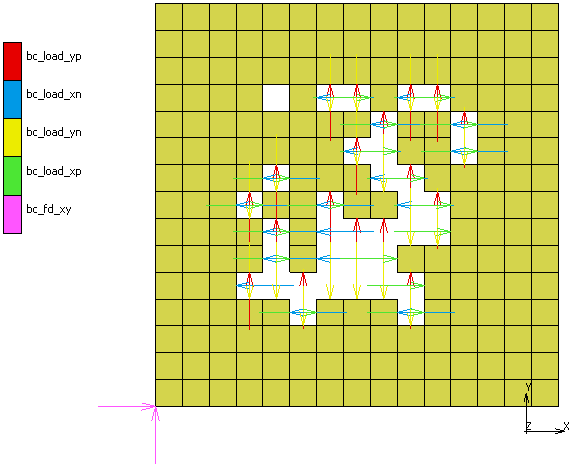
\includegraphics[width=0.5\textwidth]{unit1bc.png}
	\caption[FEM validation model of unit 1]{grid\_36\_d68df4e04590e068b46c0e75dcdf5818 FEM model with applied boundary conditions}
	\label{fig:unit1bc}
\end{figure}

\begin{figure}[H]
	\centering
	\includegraphics[width=0.5\textwidth]{unit1mod.png}
	\caption[Physical validation model of unit 1]{grid\_36\_d68df4e04590e068b46c0e75dcdf5818 physical model}
	\label{fig:unit1mod}
\end{figure}

Figure~\ref{fig:unit1def} shows comparisons between the FEM model and the physical model as the internal pressure is increased. Figure~\ref{fig:unit1over} illustrates an overlay of the FEM model deformation with the physical model's deformation. The FEM deformation is taken from step 2 of the simulation. The physical deformation is the final deformation.

\begin{figure}[H]
	\centering
	\begin{subfigure}[c]{\textwidth}
		\centering
		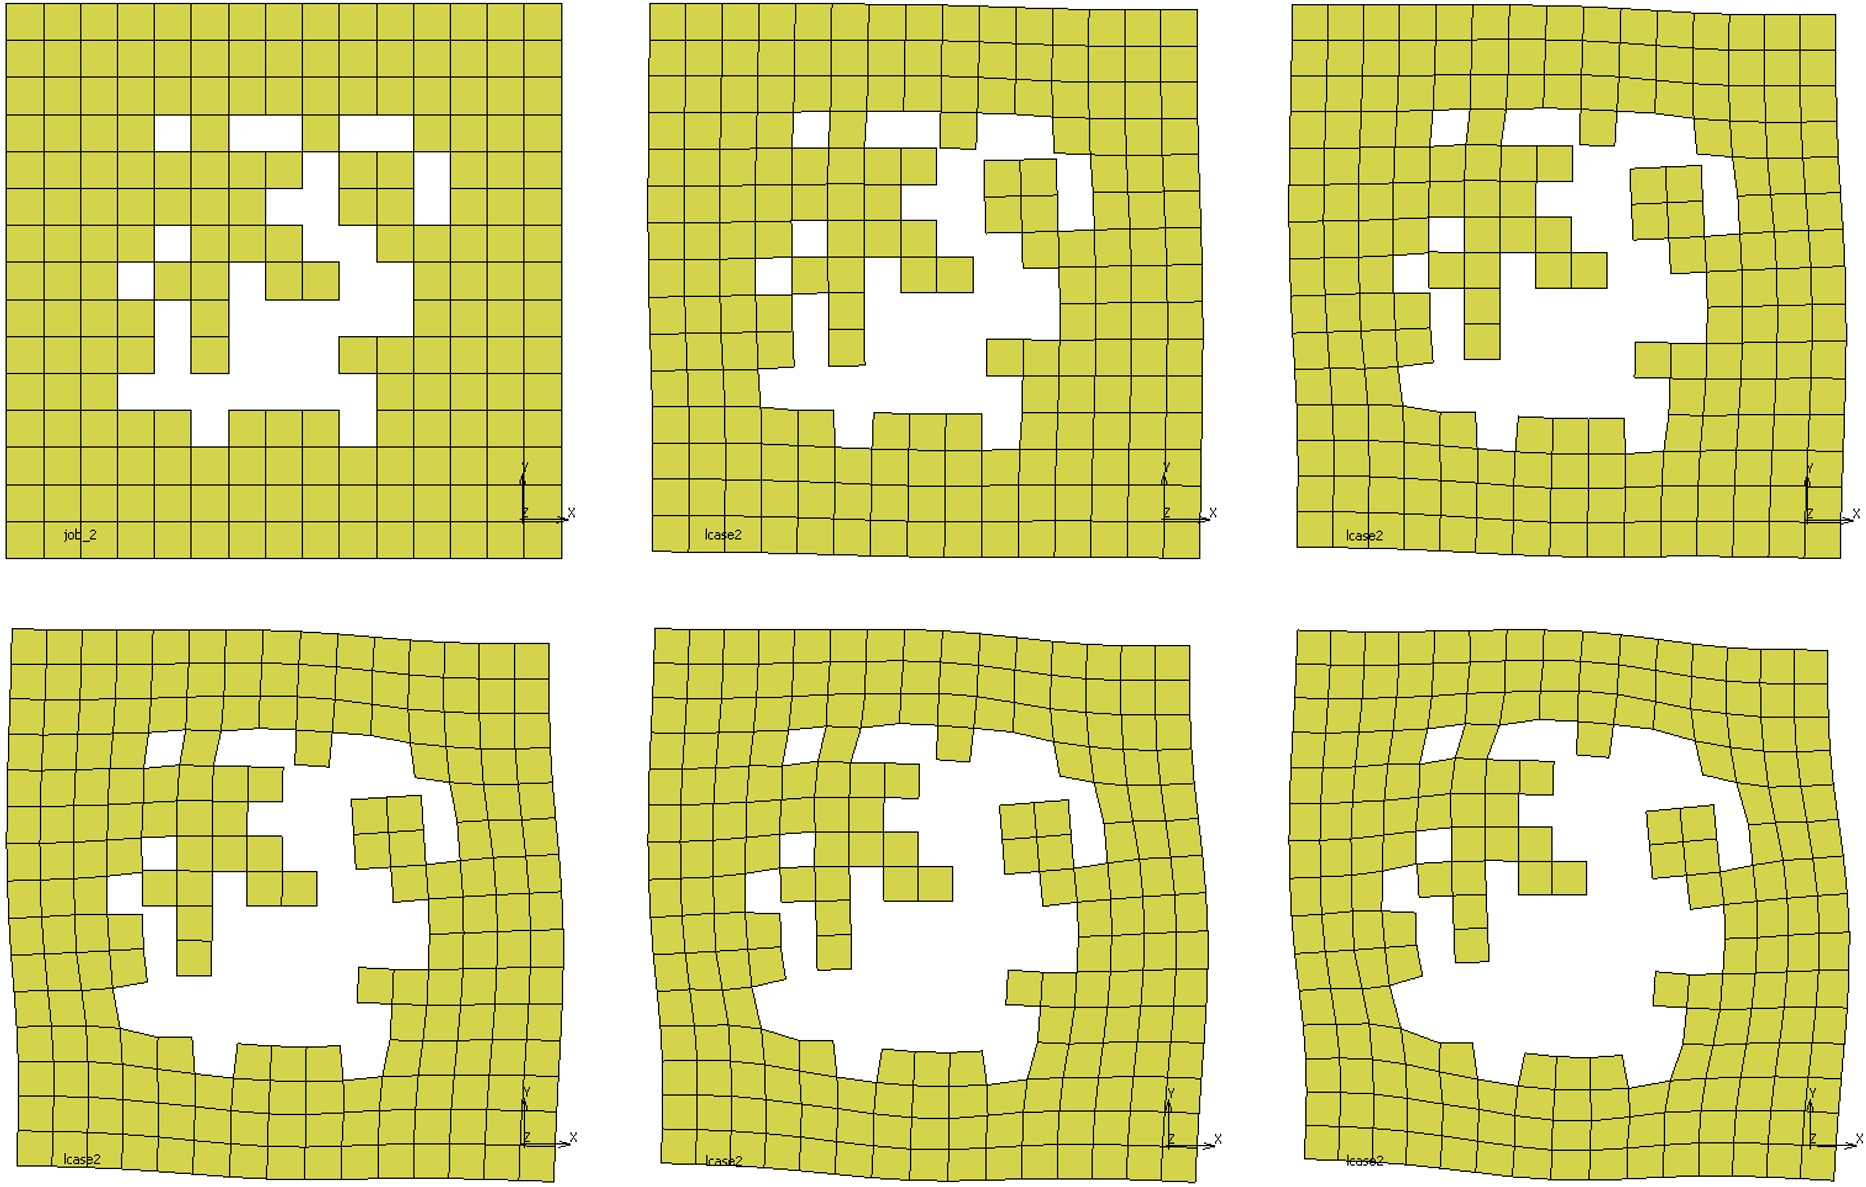
\includegraphics[width=\textwidth]{unit1deffem.png}
		\caption{FEM model deformation as internal pressure is increased. Steps 0-5 of the simulation are shown from left to right.}
	\end{subfigure}
	\hfill
	\begin{subfigure}[c]{\textwidth}
		\centering
		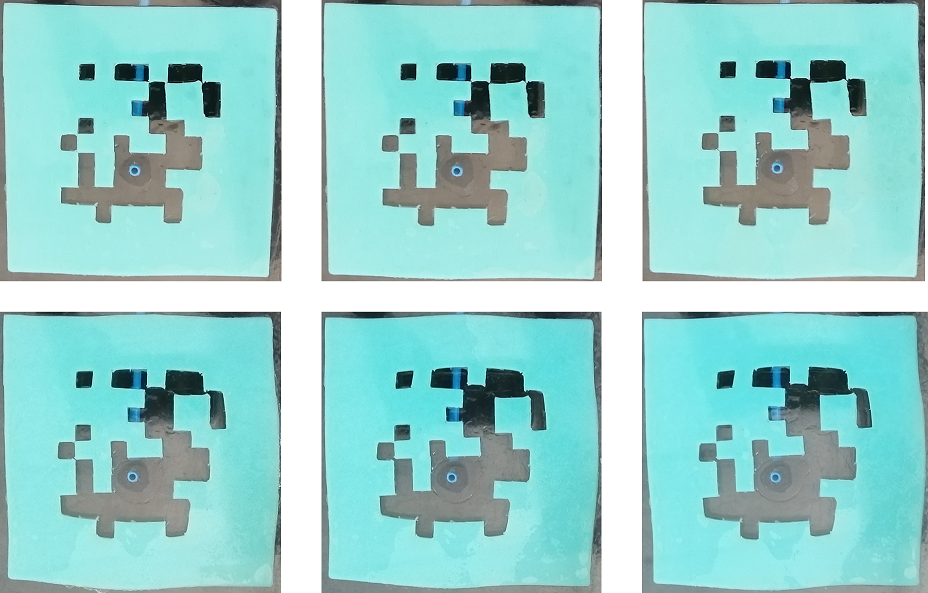
\includegraphics[width=\textwidth]{unit1defmod.png}
		\caption{Physical model deformation as internal pressure is increased}
	\end{subfigure}
	\caption[Comparison between FEM and physical models of unit 1]{Comparison between deformation of the FEM model and physical model of grid\_36\_d68df4e04590e068b46c0e75dcdf5818 as the internal pressure is increased}
	\label{fig:unit1def}
\end{figure}

\begin{figure}[H]
	\centering
	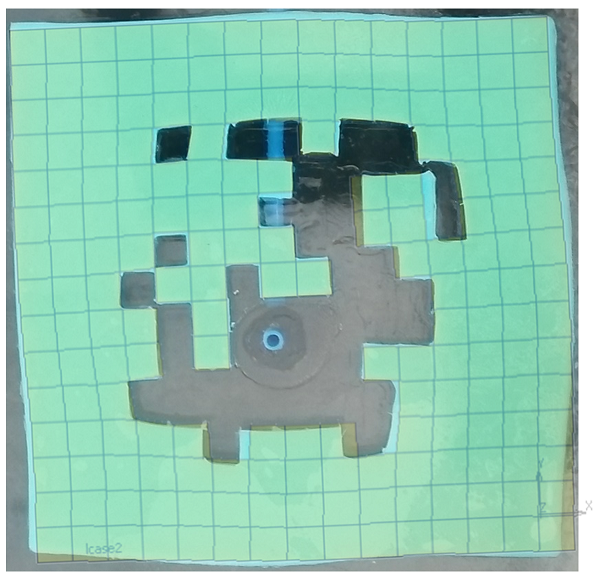
\includegraphics[width=0.8\textwidth]{unit1defover.png}
	\caption[Physical model of unit 1 overlayed with FEM model]{grid\_36\_d68df4e04590e068b46c0e75dcdf5818 physical model overlayed with FEM model at step 2 of simulation}
	\label{fig:unit1over}
\end{figure}

\subsection{Unit 2}

The second unit selected is grid\_57\_292a241d90d8d6b4753d110deca32360. This unit was selected as a linearly extending unit. This unit performs well according to the uniaxial deformation case. Cavities exist which are potentially inaccessible from the undeformed state, but become accessible as the unit inflates. The FEM model with boundary conditions is illustrated in Figure~\ref{fig:unit2bc}. The physical model is illustrated in Figure~\ref{fig:unit2mod}.

\begin{figure}[H]
	\centering
	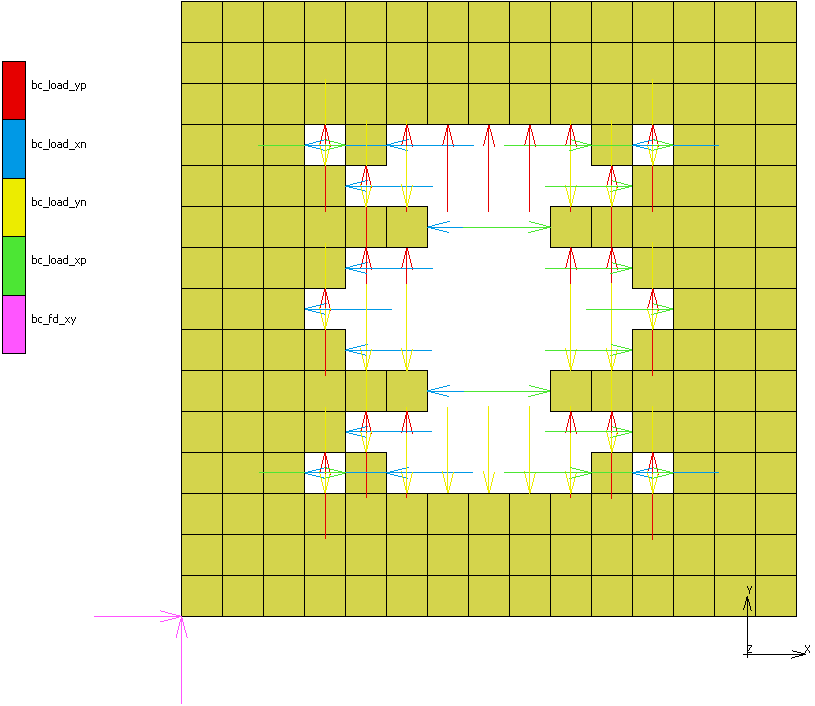
\includegraphics[width=0.5\textwidth]{unit2bc.png}
	\caption[FEM validation model of unit 2]{grid\_57\_292a241d90d8d6b4753d110deca32360 FEM model with applied boundary conditions}
	\label{fig:unit2bc}
\end{figure}

\begin{figure}[H]
	\centering
	\includegraphics[width=0.5\textwidth]{unit2mod.png}
	\caption[Physical validation model of unit 2]{grid\_57\_292a241d90d8d6b4753d110deca32360 physical model}
	\label{fig:unit2mod}
\end{figure}

Figure~\ref{fig:unit2def} shows comparisons between the FEM model and the physical model as the internal pressure is increased. Figure~\ref{fig:unit2over} illustrates an overlay of the FEM model deformation with the physical model's deformation. The FEM deformation is taken from step 3 of the simulation. The physical deformation is the final deformation.

\begin{figure}[H]
	\centering
	\begin{subfigure}[c]{\textwidth}
		\centering
		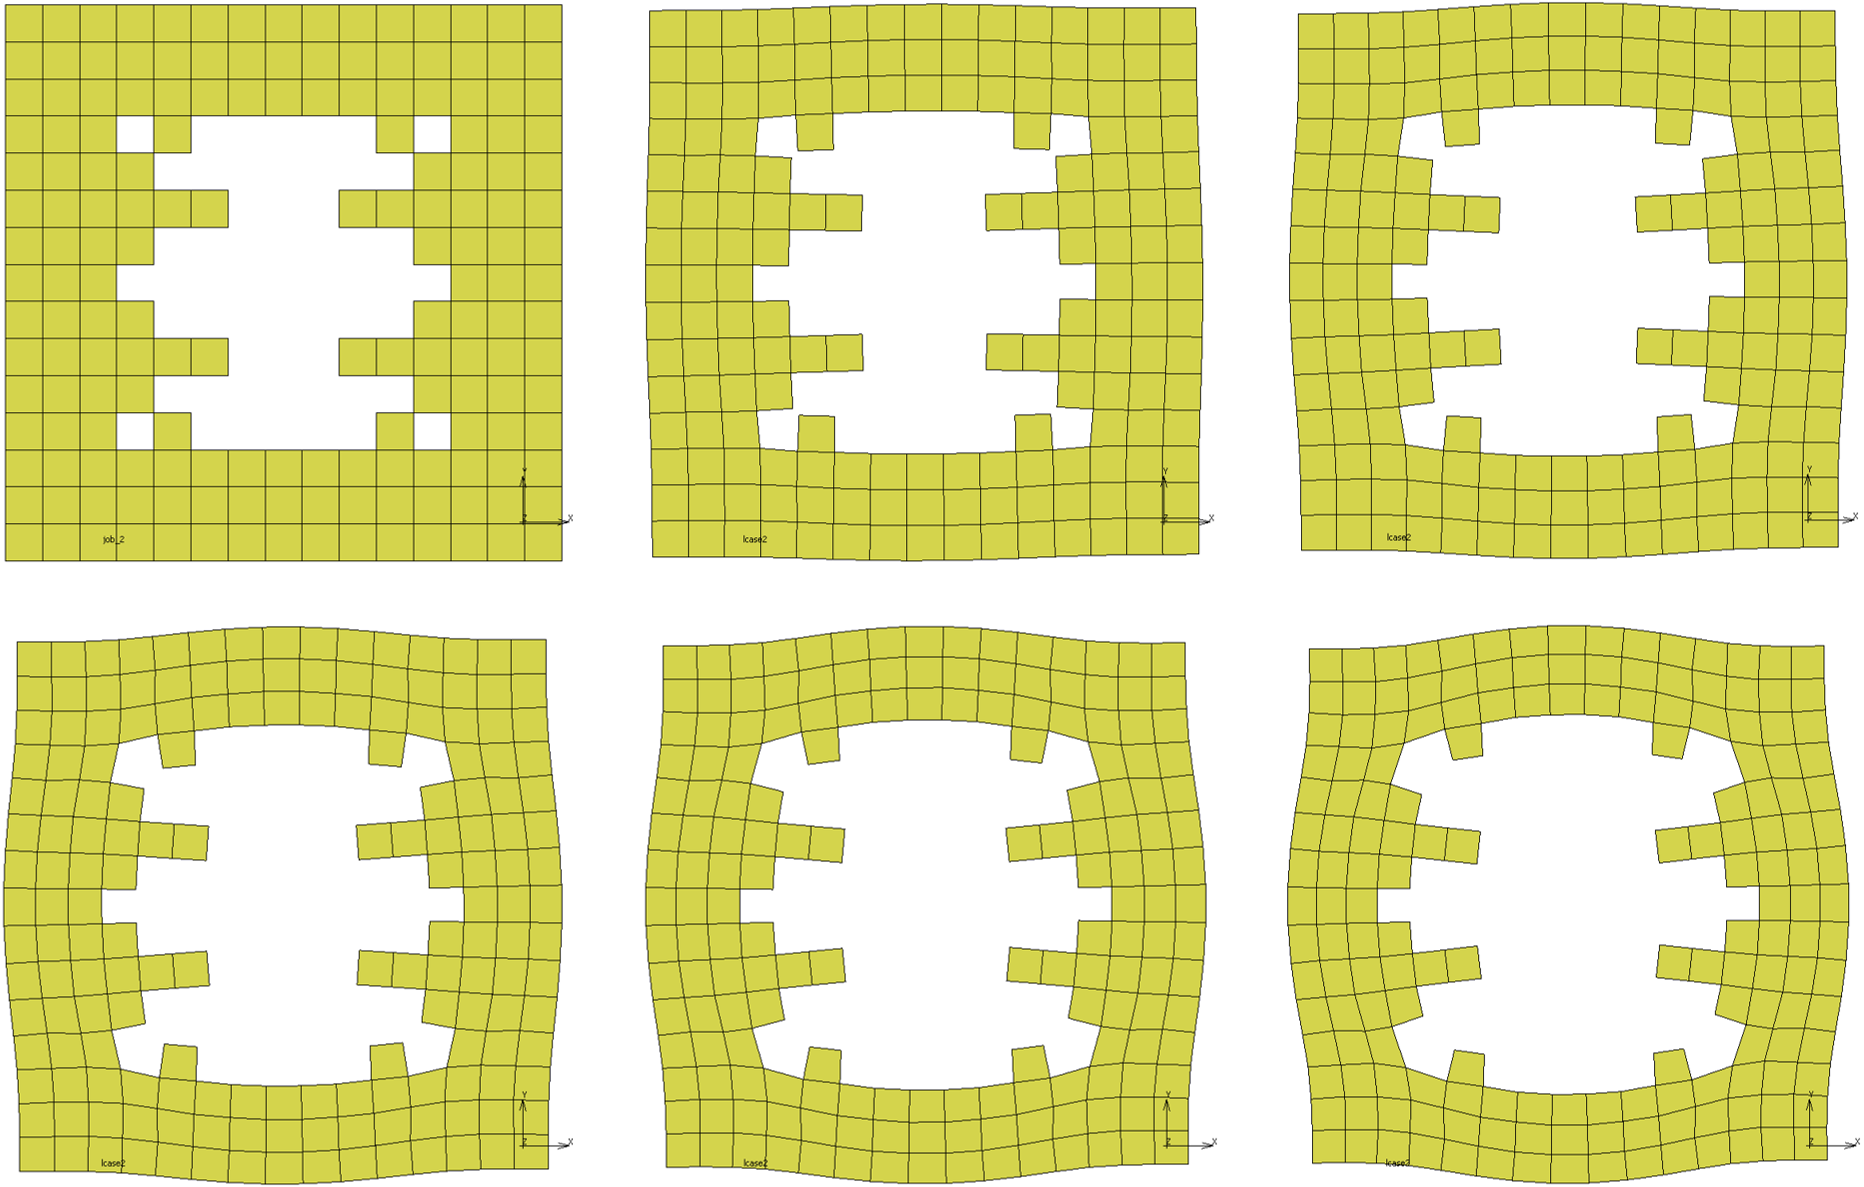
\includegraphics[width=\textwidth]{unit2deffem.png}
		\caption{FEM model deformation as internal pressure is increased. Steps 0-5 of the simulation are shown from left to right.}
	\end{subfigure}
	\hfill
	\begin{subfigure}[c]{\textwidth}
		\centering
		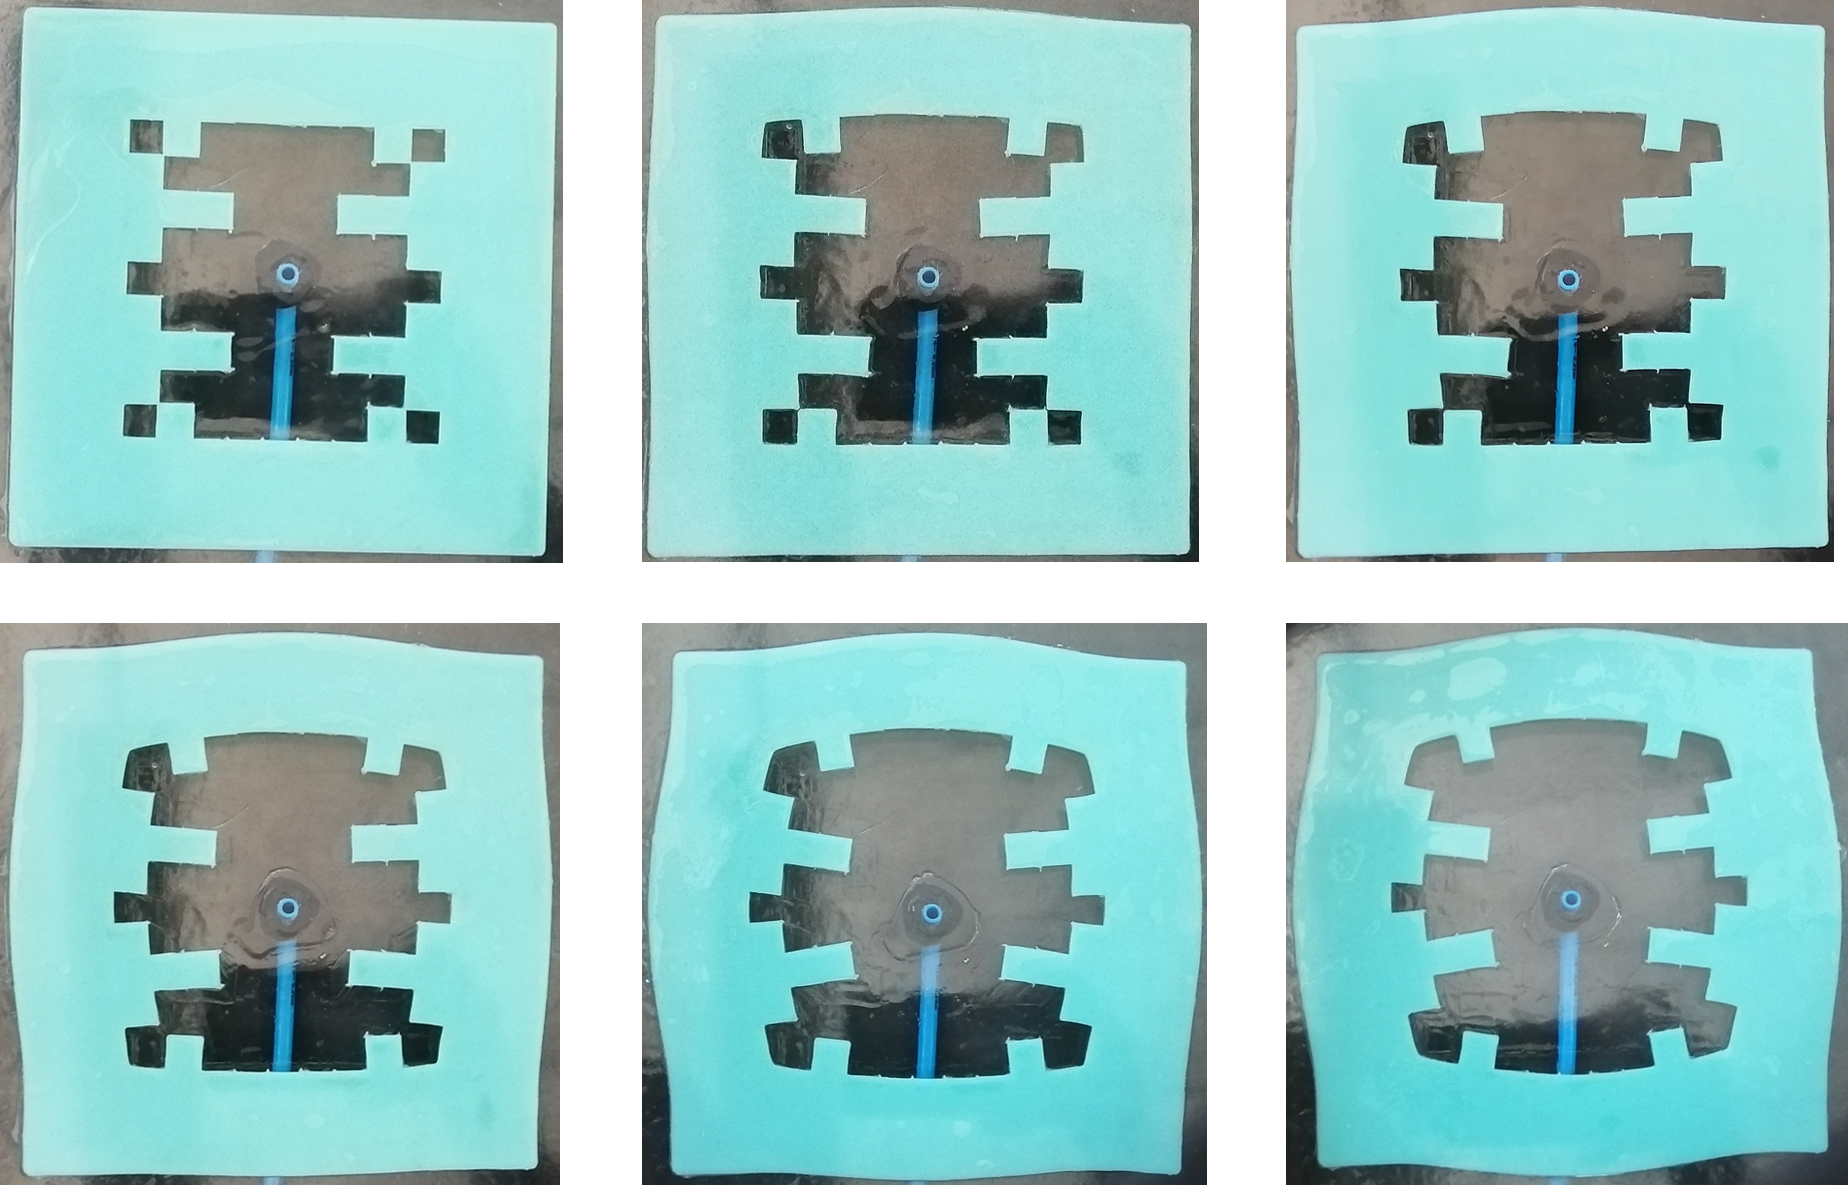
\includegraphics[width=\textwidth]{unit2defmod.png}
		\caption{Physical model deformation as internal pressure is increased}
	\end{subfigure}
	\caption[Comparison between FEM and physical models of unit 2]{Comparison between deformation of the FEM model and physical model of grid\_57\_292a241d90d8d6b4753d110deca32360 as the internal pressure is increased}
	\label{fig:unit2def}
\end{figure}

\begin{figure}[H]
	\centering
	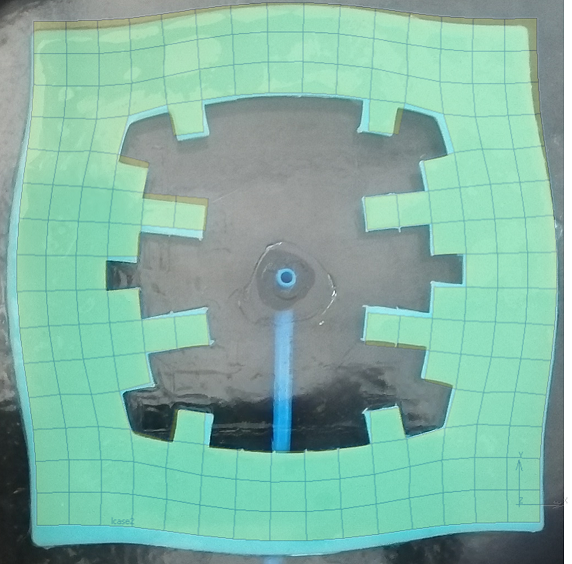
\includegraphics[width=0.8\textwidth]{unit2defover.png}
	\caption[Physical model of unit 2 overlayed with FEM model]{grid\_57\_292a241d90d8d6b4753d110deca32360 physical model overlayed with FEM model at step 4 of simulation}
	\label{fig:unit2over}
\end{figure}

\subsection{Unit 3}

The third unit selected is grid\_50\_9a02e87afe77b71561f73745d87b35bd. This unit was selected as a linearly extending unit. This unit performs well according to the uniaxial deformation case when surrounded by identical units, but performs poorly when on its own. The FEM model with boundary conditions is illustrated in Figure~\ref{fig:unit3bc}. The physical model is illustrated in Figure~\ref{fig:unit3mod}.

\begin{figure}[H]
	\centering
	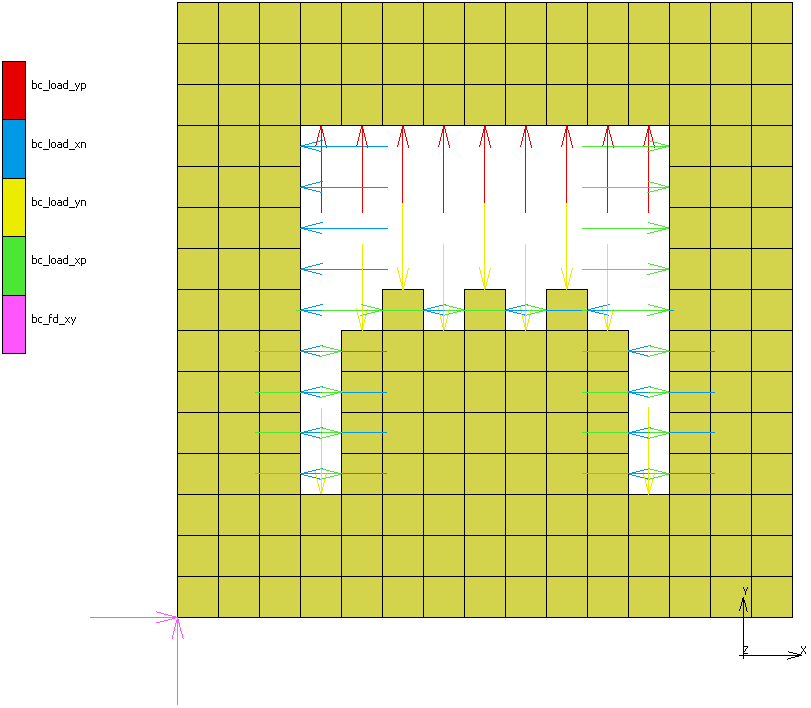
\includegraphics[width=0.5\textwidth]{unit3bc.png}
	\caption[FEM validation model of unit 3]{grid\_50\_9a02e87afe77b71561f73745d87b35bd FEM model with applied boundary conditions}
	\label{fig:unit3bc}
\end{figure}

\begin{figure}[H]
	\centering
	\includegraphics[width=0.5\textwidth]{unit3mod.png}
	\caption[Physical validation model of unit 3]{grid\_50\_9a02e87afe77b71561f73745d87b35bd physical model}
	\label{fig:unit3mod}
\end{figure}

Figure~\ref{fig:unit3def} shows comparisons between the FEM model and the physical model as the internal pressure is increased. Figure~\ref{fig:unit3over} illustrates an overlay of the FEM model deformation with the physical model's deformation. The FEM deformation is taken from step 2 of the simulation. The physical deformation is the final deformation.

\begin{figure}[H]
	\centering
	\begin{subfigure}[c]{\textwidth}
		\centering
		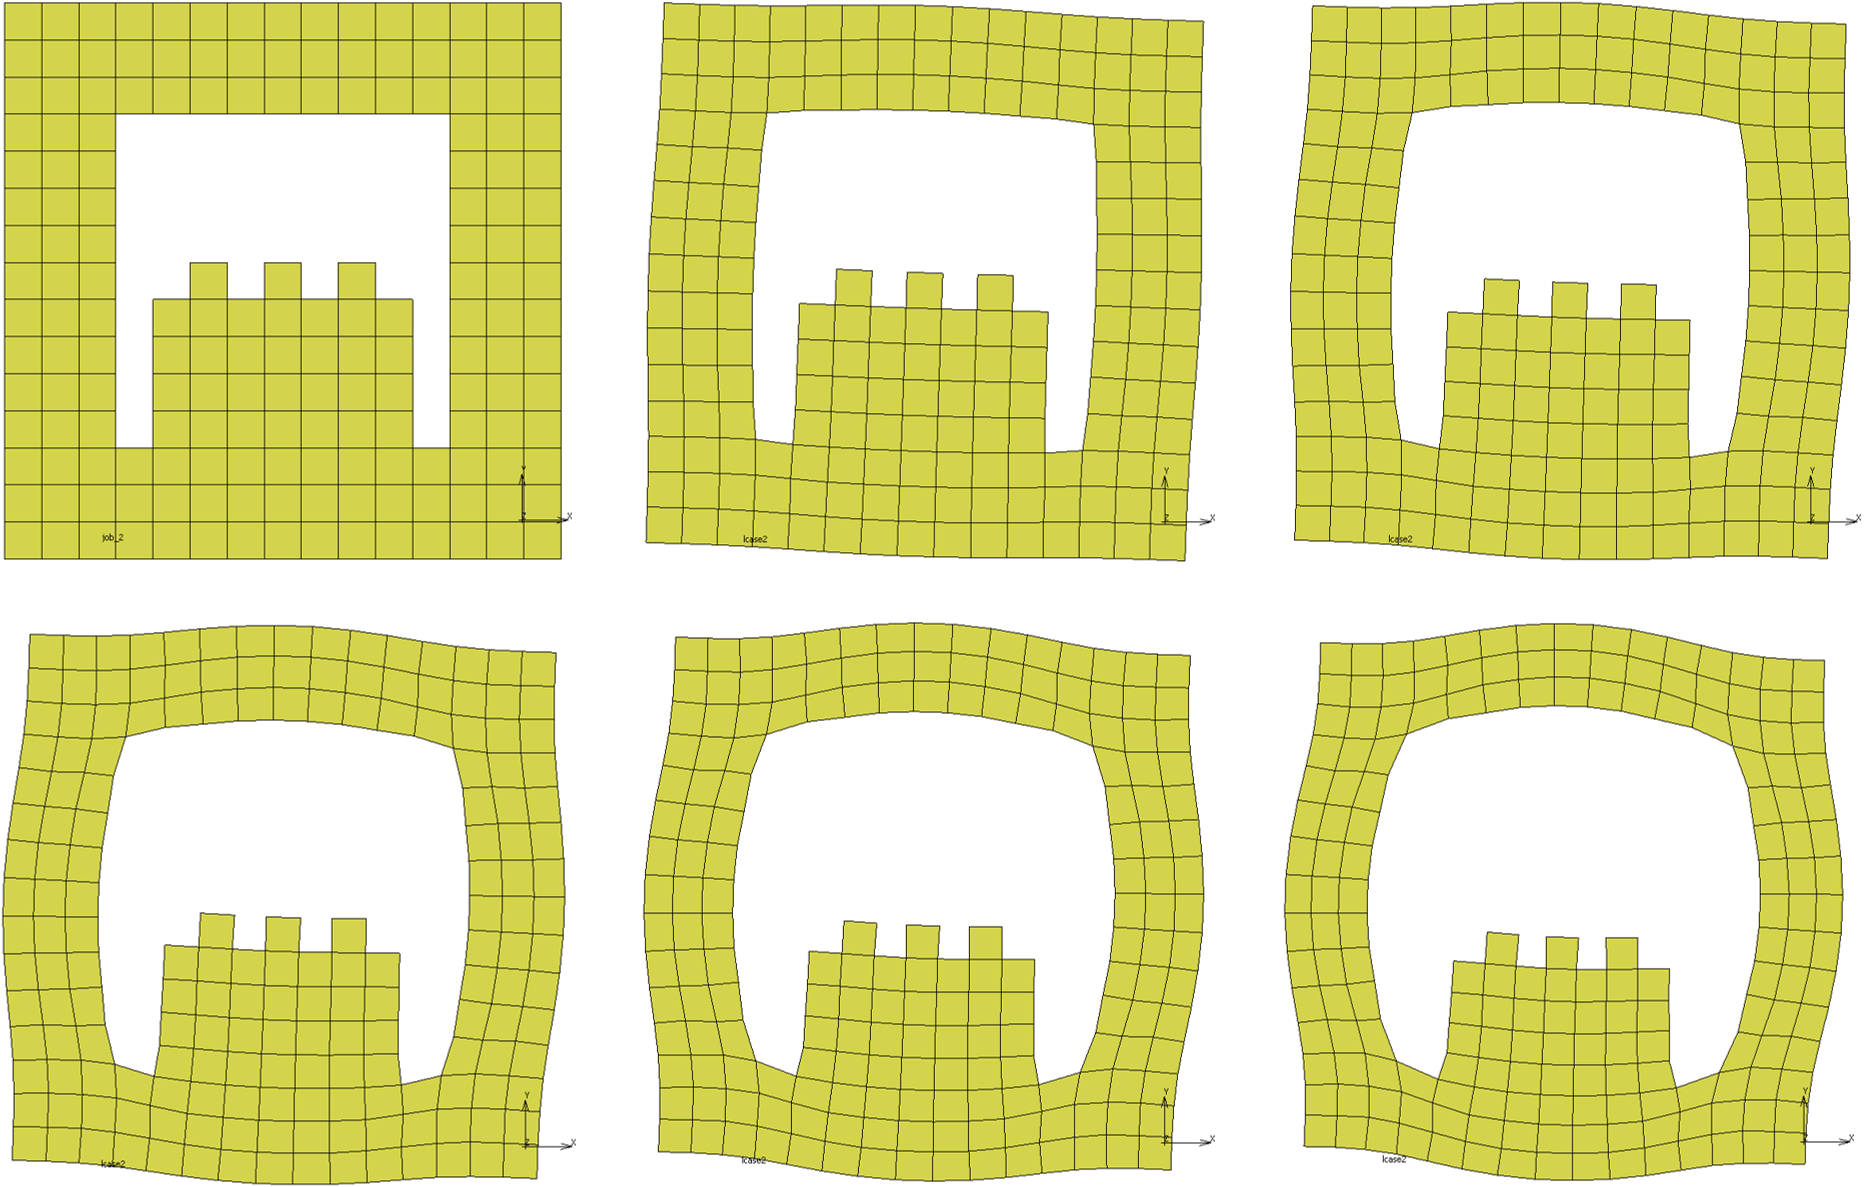
\includegraphics[width=\textwidth]{unit3deffem.png}
		\caption{FEM model deformation as internal pressure is increased. Steps 0-5 of the simulation are shown from left to right.}
	\end{subfigure}
	\hfill
	\begin{subfigure}[c]{\textwidth}
		\centering
		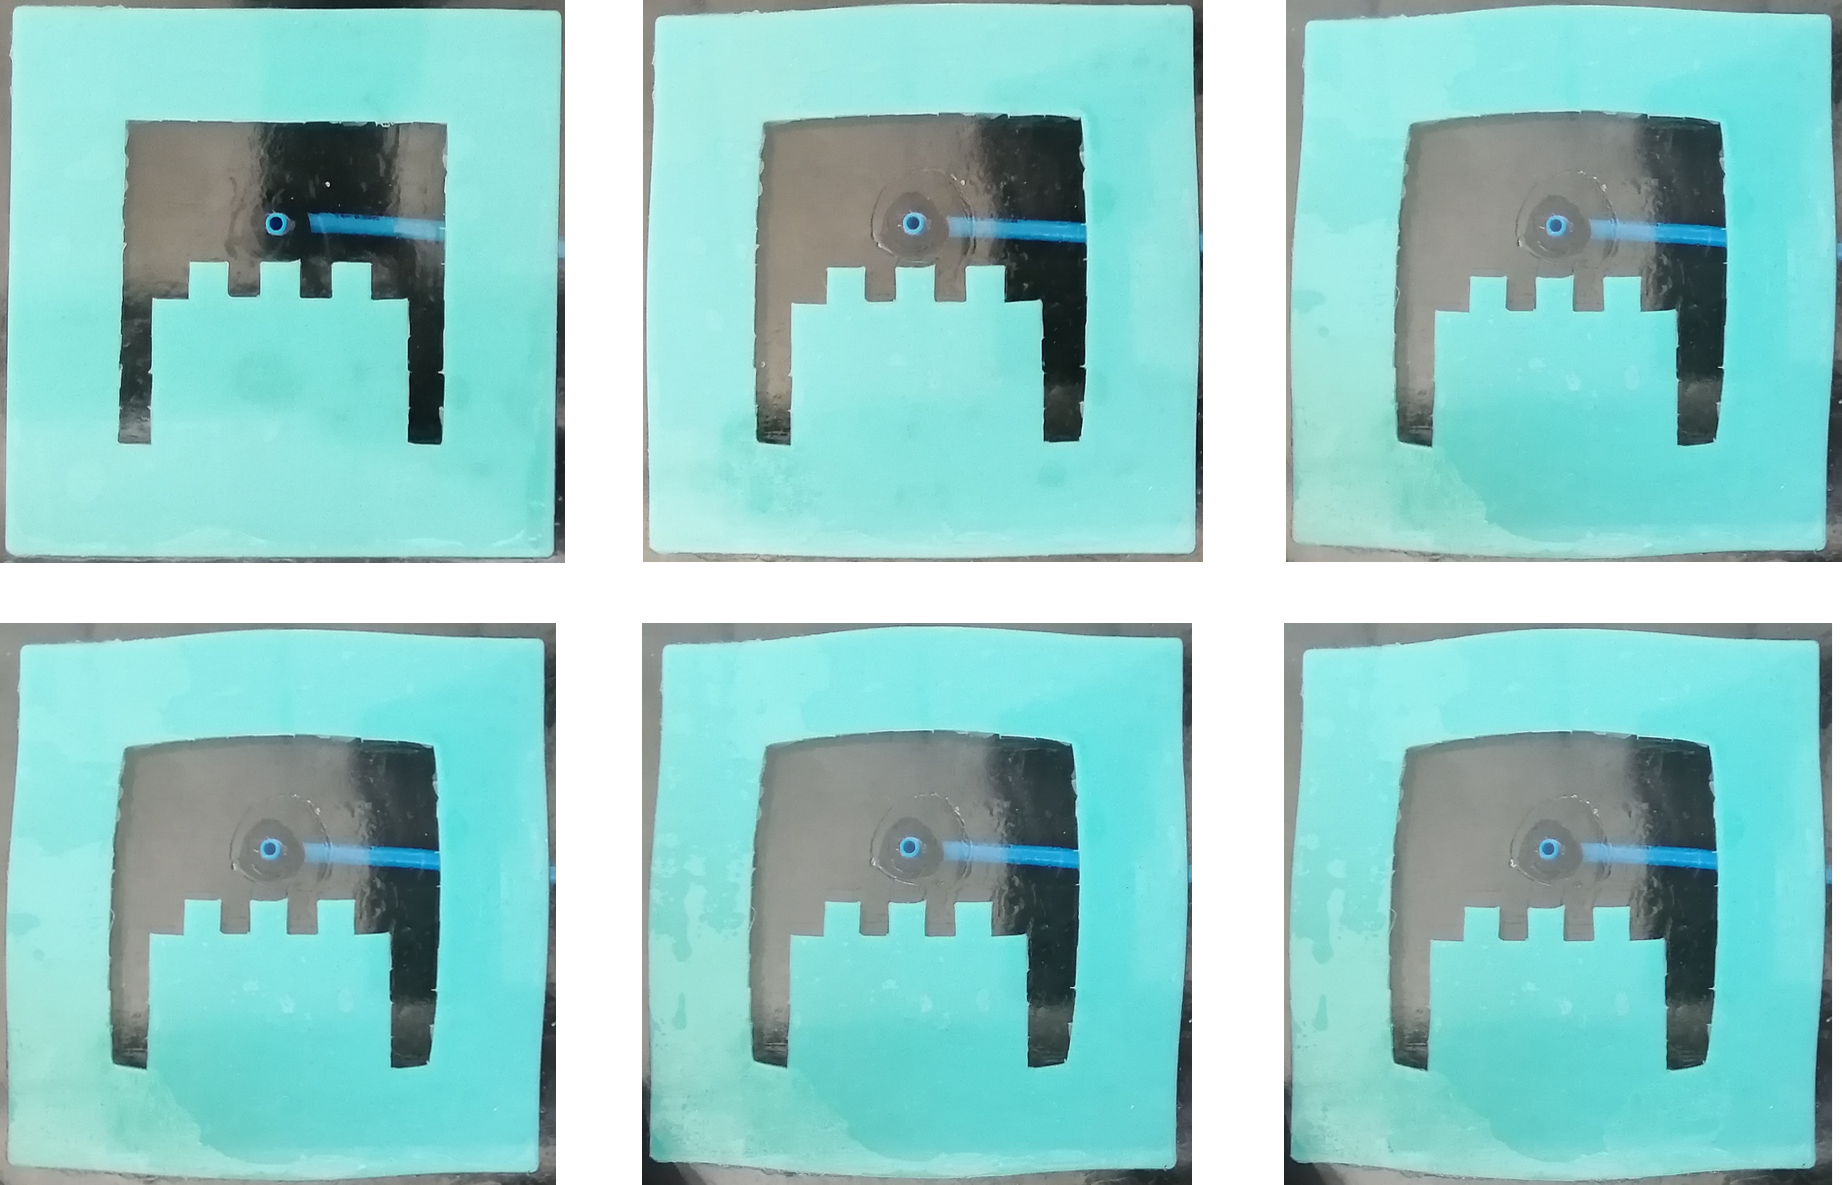
\includegraphics[width=\textwidth]{unit3defmod.png}
		\caption{Physical model deformation as internal pressure is increased}
	\end{subfigure}
	\caption[Comparison between FEM and physical models of unit 3]{Comparison between deformation of the FEM model and physical model of grid\_50\_9a02e87afe77b71561f73745d87b35bd as the internal pressure is increased}
	\label{fig:unit3def}
\end{figure}

\begin{figure}[H]
	\centering
	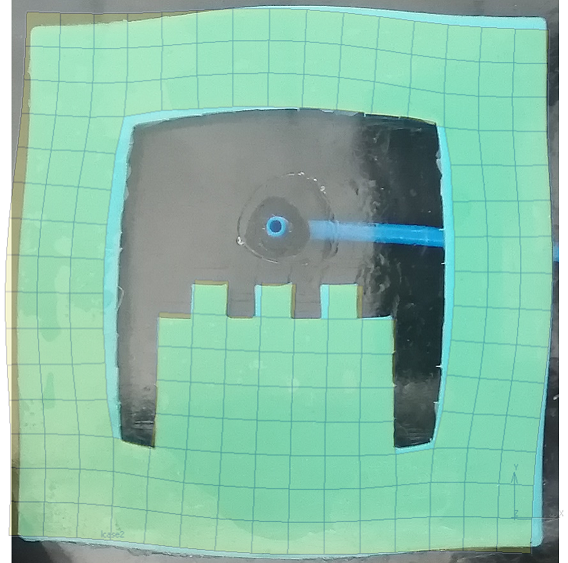
\includegraphics[width=0.8\textwidth]{unit3defover.png}
	\caption[Physical model of unit 3 overlayed with FEM model]{grid\_50\_9a02e87afe77b71561f73745d87b35bd physical model overlayed with FEM model at step 2 of simulation}
	\label{fig:unit3over}
\end{figure}

\section{Results}

The FEM models were predictive of the behaviour of the physical units. The complex internal geometries behaved as expected, with minor differences. The unit outlines closely matched the predicted outlines. The FEM models may be considered accurate predictions of the physical models. The material models as obtained by \cite{Ellis2020} may be considered accurate as well.

\section{Issues, Discrepancies and Solutions}

Some issues were encountered during model validation. Some were attempted to account for beforehand and some were unforeseen.

Mould cells were not manufactured exactly to tolerances. A number of small and large mould cells were sanded by handed to remove rough edges or protrusions and to reduce their overall size. A number of mould cells had uneven sides due to manufacturing or sanding. Material seeped into gaps between mould cells during casting. The bottom of the unit had excess material where the cast material had seeped into gaps. Excess material was carefully removed by hand but the surface was not perfectly smooth. Mould cells were laser cut. Having mould cells machined may be more costly but could result in higher quality mould cells.

Units placed between the perspex plates did not seal the internal area completely. Under higher pressures, air escaped by deforming the unit up or down against the perspex plates in order for it to escape past the unit boundary. Clamps were applied to the edges of the perspex plates in order to seal the material better. Clamps may be a necessary permanent component of the experimental setup.

The silicon-based lubricant did not decrease the friction as much as was desired. A significant amount of force was required in order to move or deform the units even when only one side was in contact with the perspex. Clamping the sides of the perspex also increased the frictional resistance, as the unit was more compressed between the two plates. It is advisable to adjust the clamp strength accordingly so as to not clamp the unit too tightly.

The uneven side of the units in combination with the air leaking, clamping and high friction is assumed to account for the discrepancies between the physical models and the FEM models.
\chapter{Conclusions}
\label{chp:C}

%%%%%%%%%%%%%%%%%%%%%%%%%%%%%%%%%%%%%%%%%%%%%%%%%%%%%%%%%%%%%%%%%%%%%%%




%==== Appendices ====================================================
%\appendix
%\appendixpage

%\chapter{Code Modification}
\label{app:CM}

A short discussion on modifying the code is provided for anyone desiring to add their own functionality. The code is available in full at:

The code may be maintained and altered as more simulations are run.

\section{Analysis Approach}

Adding a new analysis approach method may be somewhat complex. A function is available to generate an entire population according to specified 
%----------------------------------------------------------------------------
\endinput

%\include{contents/App-2}
%\include{contents/App-3}

%==== Bibliography acro's & Index ===================================
\backmatter

\bibliography{backmatter/USbib-sample}
%\listoftodos
\end{document}
